\chapter{Writing the CPU}
\lettrine{N}{ow}, we are fully armed with our equipment. It is the time to get our hands dirty and start implementing a very naive MIPS CPU.
\section{What is CPU}
Central Process Unit, a.k.a. CPU, is the most important part of computers. It is in charge of the memory loading and storing, arithmetic operations and lots of other important stuffs. Most CPUs consist of a register called program counter, which record the current instruction position in the memory; in each cycle, the CPU fetches an instruction according to the program counter and start to handling a series of events encoded in the instruction.

The CPU we are going to implement consists of five parts:
\begin{enumerate}
	\item Instruction Module: Fetch the instruction and maintain the value of the program counter.
	\item Decode Module: Decode the instruction, determine the operations to be executed and get the value of the operands from the register file.
	\item Arithmetic Unit: Execute the arithmetic operations, determine the branch targets and memory operations.
	\item Memory Module: Load and store data from and into memory.
	\item Write Back Module: Act as a transition module before register writing and branching. 
\end{enumerate}
\section{Pipeline: Why and How}
Although the functions of the CPU can be achieved within a single cycle: on each rising edge of the clock, we just fetch a new instruction and wait until all the required operations are finished, it is apparent that the cycle may become too long and inefficient. 
\begin{figure}[H]
	\centering
	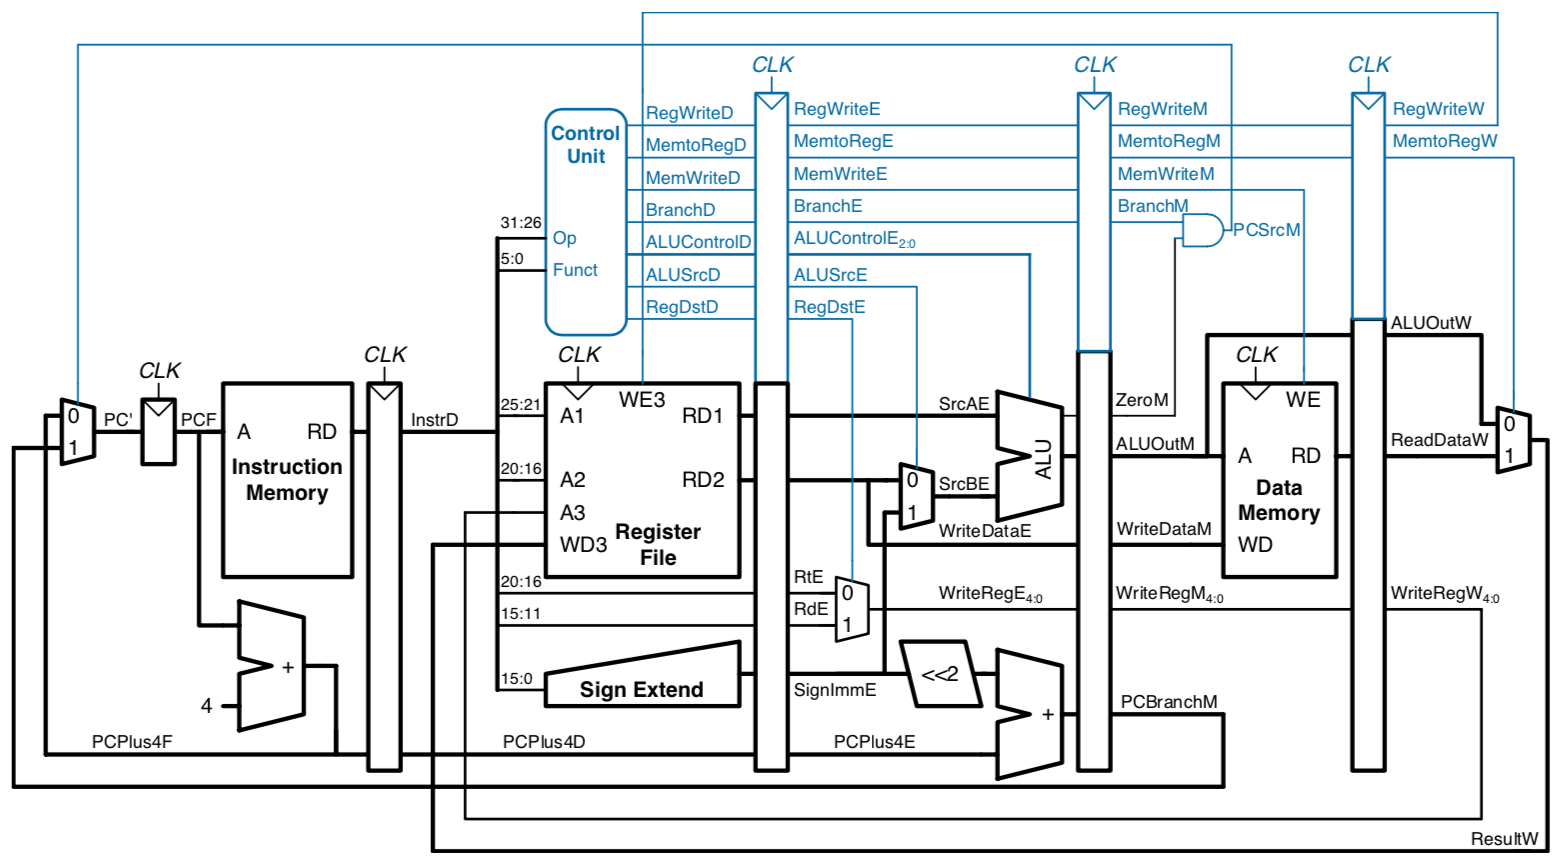
\includegraphics[width=\linewidth]{pipeline}
	\caption{Classical MIPS pipelines (without any hazard handling)}
\end{figure}
Hence, many CPUs use a strategy called pipeline which split the execution into multiple stages. Each stage stores the previous input (the output from the predecessor stage) in its register, and when the clock rises, the CPU is handling multiple instructions with different facilities. The efficiency is thus largely improved.

However, lots of new problems emerge because of the pipeline.
\subsection{Control Hazards: Branch and Jump}
Just consider the CPU shown in Figure 4.1. Without pipeline, a branch instruction triggers the branching in the single cycle and setup the new PC value within the same cycle; the next instruction to execute will always be correct. However, in the pipeline model, if the branch condition fails, everything works fine; nevertheless, when the branch condition checks and the branch instruction reaches the Write-Back stage, there will be three invalid instructions already accumulated in the pipeline. We must find a way to flush those invalid instruction.

This is actually easy: we just check the branch signal; if the branch target is set, we send a signal to all four modules before Write-Back and ask them to clear their instructions. \textbf{Notice that the memory writing should be stopped immediately while the register writing should be allowed}, because there are jumping instructions like \mintinline{asm}{jal} that will store the current PC value into a register and this operation is always valid as it arrives at the Write-Back part at the same time of the branch target.

In most CPUs, the cost of branching can be further reduced by branch prediction and moving branching checking into an earlier stage. Here, we are not going to care about these strategies and just handle the control hazards with stalling.

\subsection{Data Hazards}
There are several kinds of data hazards:
\begin{enumerate}
\item Consecutive arithmetic operations with data dependency:
\begin{minted}[linenos]{asm}
addi $a0, $a0, 1
addi $a0, $a0, 1
addi $a0, $a0, 1
\end{minted}
Notice that when the second/third instruction reaches the Arithmetic Module, the first/second instruction is at the Memory Part/Write-Back Part; which means the write-back operation is not applied. Hence, we must figure out a way to forward the result stored in Memory Part/Write-Back Part to Arithmetic Module in advance.
\item Arithmetic Operation followed by SW:
\begin{minted}[linenos]{asm}
addi $a0, $a0, 1
sw   $a0, -4($sp)
\end{minted}
In the SW case, the value of register a0 is not ready. We can simplify the handling by moving determination of write value into Arithmetic Part. Hence, using the strategy of forwarding, we can also handle this problem.

\item LW followed by Arithmetic Operation
\begin{minted}[linenos]{asm}
lw   $t0, 0($sp)
addi $t0, $t0, 1
\end{minted}
In the pipeline shown in Figure 4.1, the load value will not be ready even with forwarding. In this case, we must stall the pipeline: keep the PC value, the state of Decode Module and the Arithmetic Module unchanged (but accepting register write-back) and insert a NOP state into memory module for the next cycle while handling the current operation of loading. Therefore, in the next cycle, the second instruction is still at the Arithmetic Module while the load result reaches the Write-Back Part which makes it possible to be forwarded to ALU. 
\end{enumerate}

\subsection{Special Changes}
We made several special changes to make life easier: 
\begin{enumerate}
	\item Because we are using the BRAM structure, which means that there is one cycle delay before we can get the real data, we need to forward the ALU results to the Memory Module in the same cycle so that in the next cycle the Memory Output is exactly what the instruction in the Memory Module requires.
	\begin{minted}[linenos]{asm}
j    SOME_PLACE
sw   $zero, 4($sp)
sw   $zero, 4($sp)
	\end{minted}
	Previously, when the branch target reaches Write-Back Part, the Memory Operation hasn't taken place; however, in our case, the stall caused by branching will only prevent the second Memory Operation after branching; we need to also check the branching before we want to write something into the memory. Fortunately, this is always available since, when the instruction right after branching arrives ALU, the branching instruction is exactly at the Memory Part, we can simply check whether the branching target is set or not.
	\item There is no need to care about the Load Data Hazards as we will also forward the data together with the memory fetching result. (Thanks to BRAM delay, the extra cost is little)
\end{enumerate}
\section{Implementation}
\subsection{Instruction Module}
\subsubsection{Instruction Set}
We will only implement a very small set of MIPS instructions. Let's first write some functions to help us decode the instruction:
\begin{minted}{haskell}

-- | The Format of MIPS Instructions
data Format            
  = NoType             -- ^ NoType (Specialized for NOP Instruction)
  | RType              -- ^ R-Type Instruction Format
      (BitVector 6)    -- ^ Operation Code
      (BitVector 5)    -- ^ Register S
      (BitVector 5)    -- ^ Register T
      (BitVector 5)    -- ^ Register D
      (BitVector 5)    -- ^ Extra Infomation for Shifting Amount
      (BitVector 6)    -- ^ Function Code
  | IType              -- ^ I-Type Instruction Format
      (BitVector 6)    -- ^ Operation Code
      (BitVector 5)    -- ^ Register S
      (BitVector 5)    -- ^ Register T
      (BitVector 16)   -- ^ Immediate Value
  | JType              -- ^ J-Type Instruction Format 
      (BitVector 6)    -- ^ Operation Code
      (BitVector 26)   -- ^ Jump Target
  deriving Show
\end{minted}
We will first recognize the instruction format and then transform it into each recognized instruction.
\begin{minted}{haskell}
decodeFormat :: BitVector 32 -> Format
decodeFormat 0 = NoType
decodeFormat vec =
    let opcode = slice d31 d26 vec
    in case opcode of
       0 ->
           pure RType 
               <*> (slice d31 d26)
               <*> (slice d25 d21) 
               <*> (slice d20 d16) 
               <*> (slice d15 d11) 
               <*> (slice d10 d6) 
               <*> (slice d5 d0) 
                $  vec
      code | code == 0b000010 || code == 0b000011 ->
           pure JType 
               <*> (slice d31 d26) 
               <*> (slice d25 d0) 
                $ vec
      _ ->
           pure IType 
               <*> (slice d31 d26) 
               <*> (slice d25 d21) 
               <*> (slice d20 d16) 
               <*> (slice d15 d0) 
                $  vec
\end{minted}
The format decode is trivial:
\begin{itemize}
	\item An all-zero instruction is an NOP;
	\item Otherwise, instructions with 0 opcode will be dispatched into R-Format;
	\item Instructions with special jumping opcode will be dispatched into J-Format;
	\item Other instructions are in the I-Format
\end{itemize}
After the format is determined, we can then transform instructions into our inner forms:

\begin{minted}{haskell}
type Register = Unsigned 5
data Instruction
    = NOP
    | ADD Register Register Register
    | ADDI Register Register (Signed 16)
    | ADDU Register Register Register
    | ADDIU Register Register (Unsigned 16)
    | SUB Register Register Register
    | SUBU Register Register Register
    | AND Register Register Register
    | ANDI Register Register (BitVector 16)
    | NOR Register Register Register
    | OR Register Register Register
    | ORI Register Register (BitVector 16)
    | XOR Register Register Register
    | XORI Register Register (BitVector 16)
    | BEQ Register Register (Signed 16)
    | BNE Register Register (Signed 16)
    | SLT Register Register Register
    | SLTI Register Register (Signed 16)
    | SLTU Register Register Register
    | SLTIU Register Register (Unsigned 16)
    | LW Register Register (Signed 16)
    | SW Register Register (Signed 16)
    | SLL Register Register (Unsigned 5)
    | SRL Register Register (Unsigned 5)
    | SRA Register Register (Unsigned 5)
    | SLLV Register Register Register
    | SRLV Register Register Register
    | SRAV Register Register Register
    | J (Unsigned 26)
    | JAL (Unsigned 26)
    | JR (Unsigned 5)
    deriving Show
    deriving Generic
    deriving NFDataX
\end{minted}
We do not provide the function \mint{haskell}{decodeTyped :: Format -> Instruction} here as it should be easy to write and just require some repeated works to recognize the instruction based on the opcode and the function code.

Just mention a small trick: to reduce code repetition, you can use the Applicative property of Readers):
\begin{minted}{haskell}
t1 (x, _, _) = x
t2 (_, y, _) = y
t3 (_, _, z) = z
makeType func = pure func <*> unpack . t1 <*> unpack . t2 <*> unpack . t3
-- then you can just write something like:
case fn of
    0b100000 -> (makeType ADD) (rs, rt, rd)
    0b100001 -> (makeType ADDU) (rs, rt, rd)
    0b100100 -> (makeType AND) (rs, rt, rd)
    -- more cases ...
\end{minted}
Please notice that for most R instructions, we will keep the format as \mintinline{haskell}{ADD rs rt rd}, but for those shift related operations, the format will be \mintinline{haskell}{SLL rd rt sa}; those I instructions adapts the format of \mintinline{haskell}{ADDI rs rt imm}.
\subsubsection{The Instruction RAM}
We will use BRAM to implement the instruction memory space. The memory itself is quite simple, we just use the  \mintinline{haskell}{blockRamFile} function to achieve the goal
\begin{minted}[breaklines]{haskell}
instrRAM' 
  ::  HiddenClockResetEnable dom
  => Signal dom MemAddr
  -> Signal dom (BitVector 32)
instrRAM' = (flip $ blockRamFile d512 "instructions.bin") $ pure Nothing

instrRAM 
  :: Clock System
  -> Reset System
  -> Enable System
  -> Signal System MemAddr
  -> Signal System (BitVector 32)
instrRAM = exposeClockResetEnable instrRAM'
\end{minted}
\subsubsection{Instruction Module Interface}
Now we must think carefully of what we are going to in this module:
\begin{enumerate}
	\item We need to maintain the value of program counter, if no branching happens, we just increase it; otherwise, we set the counter to the branch target immediately.
	\item On Each cycle, we will need to output two things: an instruction and (PC + 1) (one plus the instruction index). As BRAM has a delay effect, the current PC in this cycle is exactly the value we want, hence we do not need to make an extra addition to the counter.
	\item When stall happens, output an NOP. As the branch target is set immediately, there is no need to keep the old PC value.
\end{enumerate}
With these ideas, we can come out the following design:
\begin{figure}[H]
	\centering
	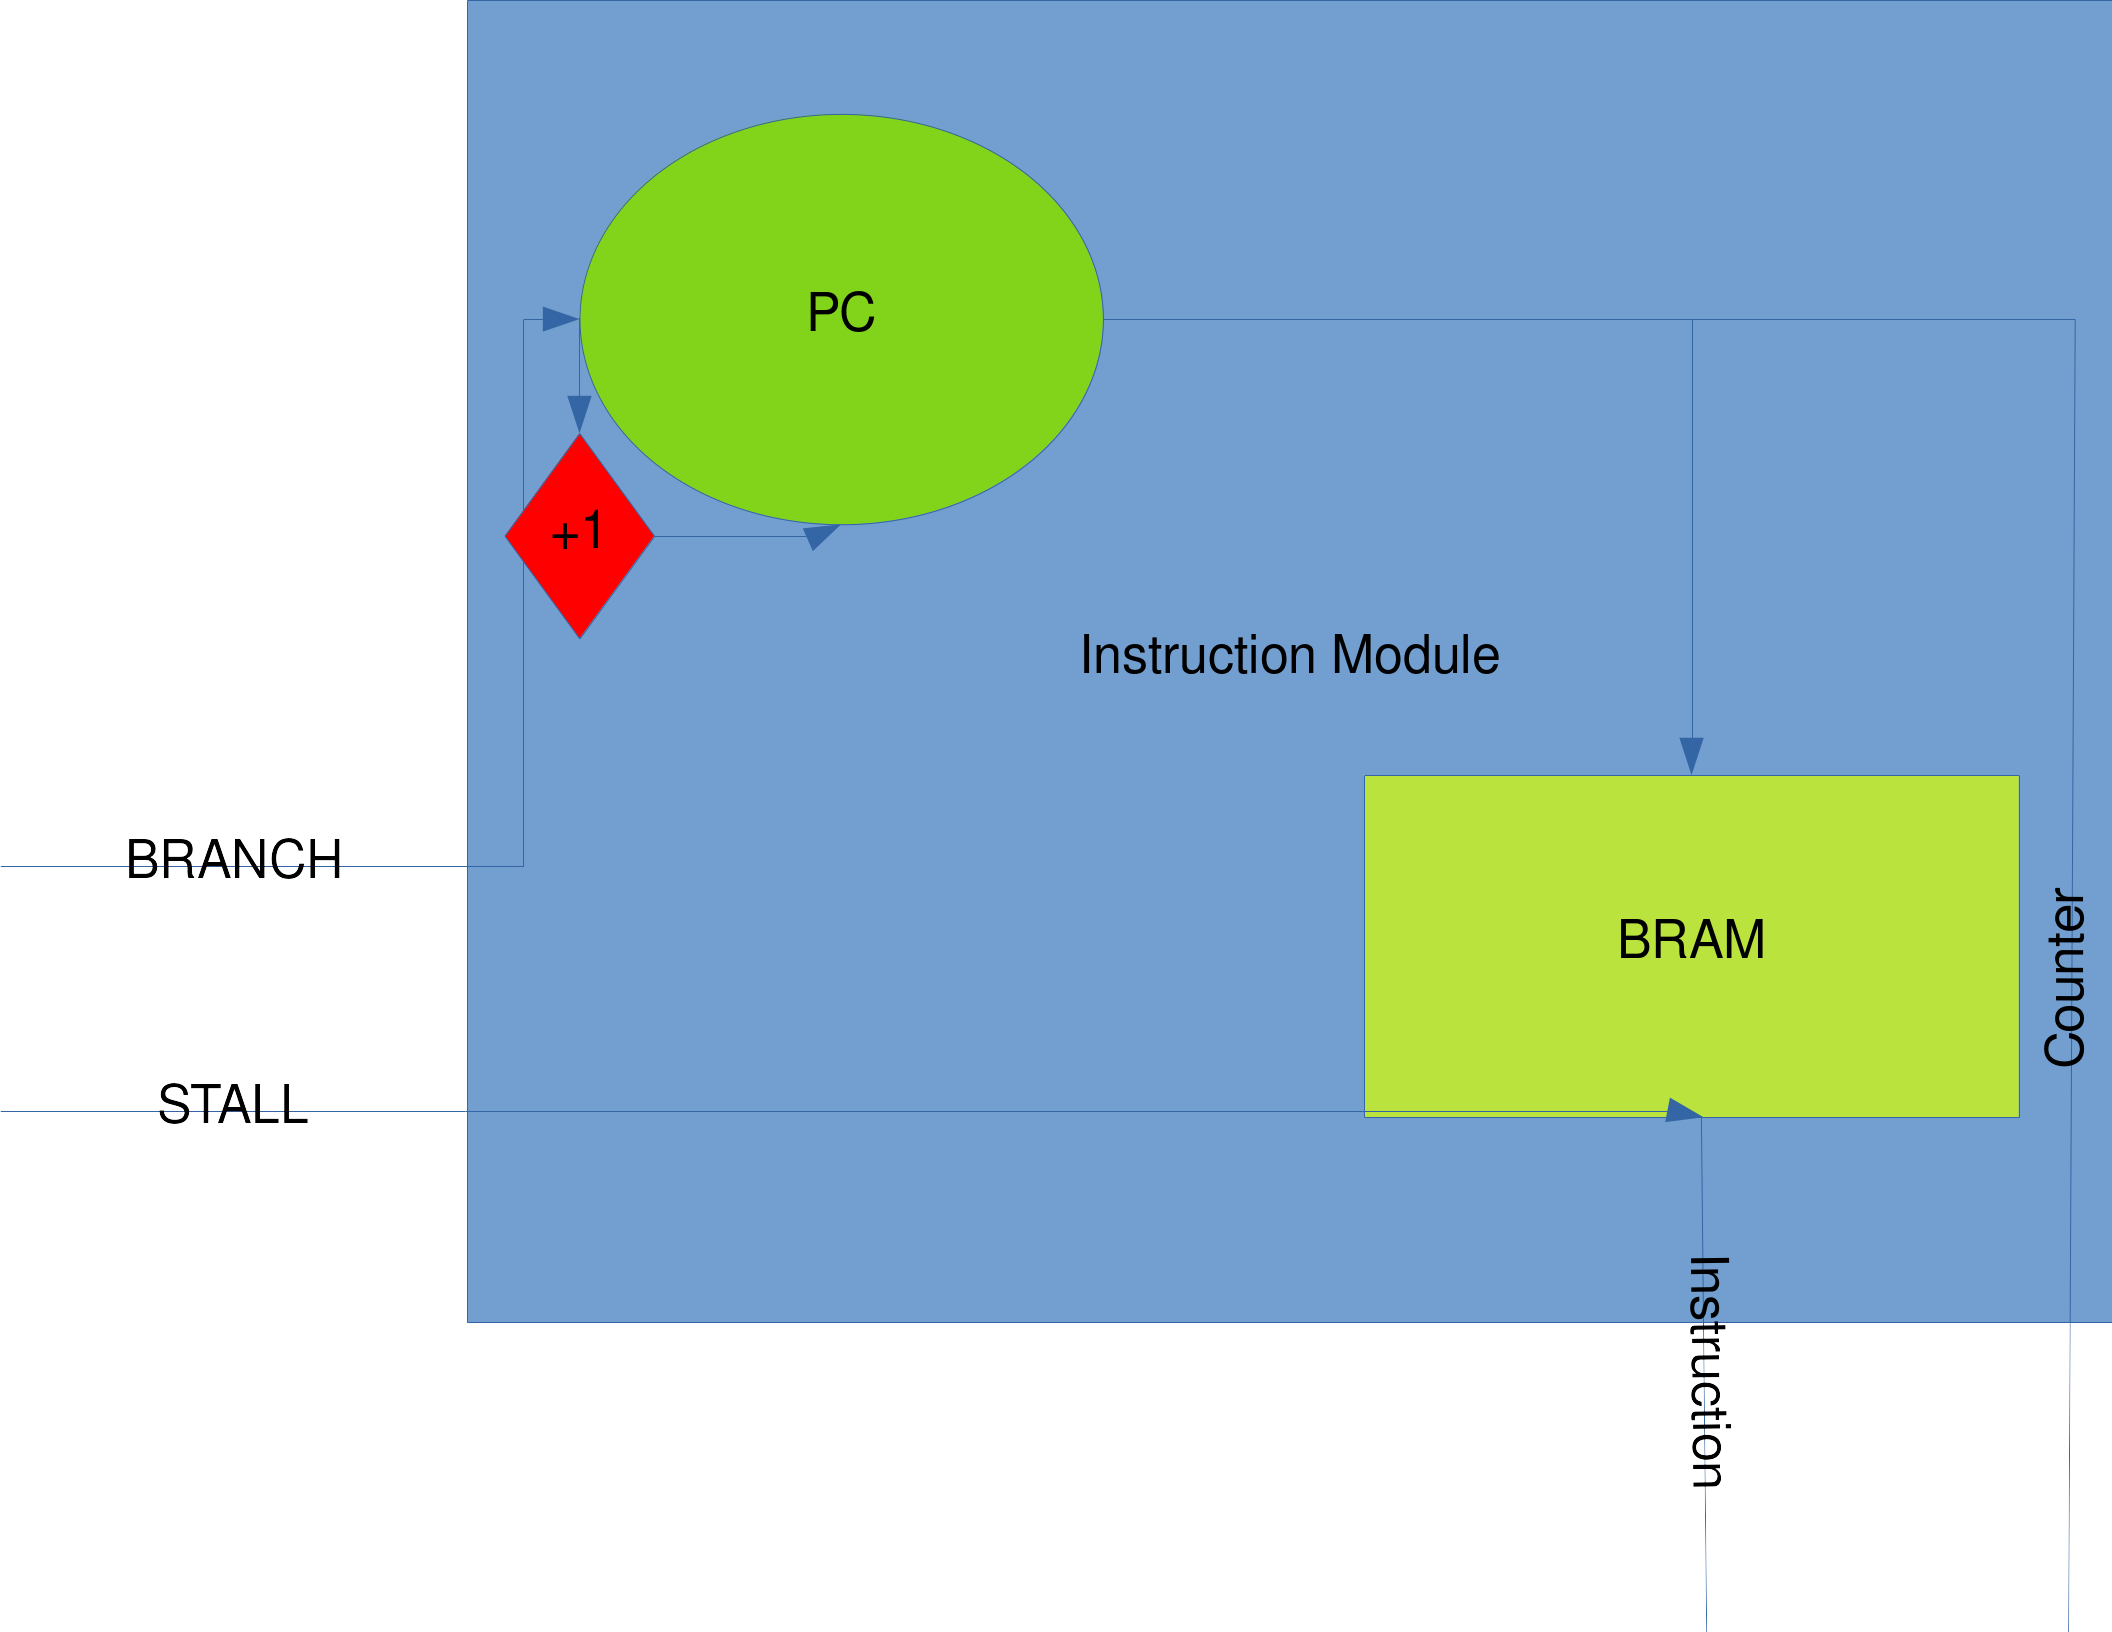
\includegraphics[width=\linewidth]{im}
	\caption{Instruction Module Diagram}
\end{figure}
Let's first maintain the PC value using a Mealy Machine:    
\begin{minted}[breaklines]{haskell}
type PCInput = Maybe (Unsigned 32)
programCounterT 
  :: Unsigned 32 
  -> PCInput
  -> (Unsigned 32, Unsigned 32)
programCounterT state (Just t) = (t + 1, t)
programCounterT state _ = (state + 1, state)

programCounter 
  :: HiddenClockResetEnable dom
  => Signal dom PCInput
  -> Signal dom (Unsigned 32)
programCounter = mealy programCounterT 0
\end{minted}
As you can see, unless the branch target is set, the PC just behaves as a monotonic counter.
\begin{minted}[breaklines, linenos]{haskell}
{-# ANN pcModule
    (Synthesize{t_name = "InstructionModule",
        t_inputs =
          [PortName "CLOCK", PortName "RESET", PortName "ENABLE", PortName "STALL", PortName "BRANCH"],
        t_output =
          PortProduct "PC" [PortName "INSTRUCTION", PortName "VALUE"]})
    #-}

pcModule 
  :: Clock System
  -> Reset System
  -> Enable System
  -> Signal System Bool
  -> Signal System (Maybe (Unsigned 32))
  -> Signal System (Instruction, (Unsigned 32))
pcModule clk rst enable stall br = bundle (instr, next)
  where
    programCounter' = (exposeClockResetEnable programCounter) clk rst enable
    next = programCounter' $ br
    ram = instrRAM clk rst enable next
    ram' = decodeTyped . decodeFormat <$> ram
    instr' op ram =
      case op of
        False -> ram
        True -> NOP
    instr = instr' <$> stall <*> ram'
\end{minted}
If you are not familiar with Haskell, just notice that $<\$>, <*>$ are the operators using the Applicative property of Signal to lift a function of \mintinline{haskell}{f :: a -> b -> c} type onto \mintinline{haskell}{f :: Signal dom a -> Signal dom b -> Signal dom c}, so that we can transform combinatorial logic into a sequential form.
The data flow is simple:
\begin{enumerate}
	\item Get the current counter with branch flag
	\item Get the memory output and set the next address to fetch
	\item Decode the output
	\item Check the stall condition and output the instruction and PC value
\end{enumerate}
Now we can happily generate the Verilog code for this module, try it!

\subsection{Decode Module}
\subsubsection{Register File}
Decode Module contains the Register File which is in charge of maintaining the register value. Let us first take a look at these definitions.
As the logic relation is a little bit complicated, we can use State Monad to construct the state machine for the Register File.
\begin{minted}[breaklines, linenos]{haskell}
type Reg = BitVector 32

type RegNo = Unsigned 5

registerFileS 
  :: ( RegNo -- rs
     , RegNo -- rt
     , Maybe (RegNo, Reg) -- write register
     )
  -> State (Vec 32 Reg) (Reg, Reg)
registerFileS (reg0, reg1, writePair)  = do
  regs <- get
  let newS =
        case writePair of
          Nothing -> regs
          Just (a, b) ->
            if a /= 0
            then replace a b regs
            else regs
      res0 = newS !! reg0
      res1 = newS !! reg1
  put newS
  return (res0, res1)

{-# ANN registerFile
    (Synthesize
      { t_name = "RegisterFile"
      , t_inputs =
        [ PortName "CLOCK"
        , PortName "RESET"
        , PortName "ENABLE"
        , PortProduct "RF" 
          [ PortName "RS"
          , PortName "RT"
          , PortName "WRITE"
          ]
        ]
      , t_output = 
        PortProduct "RF" 
          [ PortName "RSV"
          , PortName "RTV"
          ]
      }
    )
#-}

registerFile 
  :: Clock System
  -> Reset System
  -> Enable System
  -> Signal System (RegNo, RegNo, Maybe (RegNo, Reg))
  -> Signal System (Reg, Reg)
registerFile = exposeClockResetEnable $ asStateM registerFileS (replicate d32 0)
\end{minted}
The Register File takes three input: two register indices to fetch and one register write serial consists of register number and target value. The outputs are the values of required registers. Here we use read-after-write strategy to make sure that the fetched data is the latest.

\subsubsection{Control Unit}
Now comes one of the most tedious part of the entire CPU, the Control Unit. It extract the information from the instruction and separate them for further execution.

The extraction is not stateful, to reduce the complexity, we can argue this part in the combinatorial form and lift it later. 

Here we are going to define lots of data format for later uses:
 
\begin{itemize}
	\item \mintinline{haskell}{MemoryOperation}: this data tags the operation on the RAM: none, read or write:
	\begin{minted}[breaklines]{haskell}
data MemoryOperation
  = MemNone
  | MemLoad
  | MemWrite
deriving (Generic)
deriving (NFDataX)
deriving (Show)
	\end{minted}
	\item \mintinline{haskell}{BranchFlag}: Four types: no-branching, branch-on-equal, branch-on-different, jump; because conditional branching uses up two operands, we need additional field to carry the branching difference.
\begin{minted}[breaklines]{haskell}
data BranchFlag
  = NoBranch
  | BranchEQ (BitVector 32)
  | BranchNE (BitVector 32)
  | Jump
  deriving (Generic)
  deriving (NFDataX)
	\end{minted}
  \item \mintinline{haskell}{ALUOperation}: Defines the ALU Operations, those add, sub, set, right shift operations are accompanied with an extra bit to tag whether the data is signed or not.
\begin{minted}[breaklines]{haskell}
data ALUOperation
  = ALUAdd Bool
  | ALUSub Bool
  | ALUAnd
  | ALUNor
  | ALUOr
  | ALUXor
  | ALUSet Bool
  | ALUShiftL
  | ALUShiftR Bool
  | ALUNone
deriving (Generic)
deriving (NFDataX)
	\end{minted}
\end{itemize}
Now, we can write some functions to dispatch these flags. First, we can check whether there is a need of register writing. The correct register to write may vary with different instructions. One special case is the JAL instruction, which requires the update of register ra.
\begin{minted}[breaklines]{haskell}
writeRegister 
  :: HiddenClockResetEnable dom
  => Signal dom Instruction
  -> Signal dom (Maybe (Unsigned 5))
writeRegister = fmap writeRegister'
  where
    writeRegister' inst =
      case inst of
        ADD   _  _  rd -> Just rd
        ADDI  _  rt _  -> Just rt
        ADDU  _  _  rd -> Just rd
        ADDIU _  rt _  -> Just rt
        SUB   _  _  rd -> Just rd
        SUBU  _  _  rd -> Just rd
        AND   _  _  rd -> Just rd
        ANDI  _  rt _  -> Just rt
        NOR   _  _  rd -> Just rd
        OR    _  _  rd -> Just rd
        ORI   _  rt _  -> Just rt
        XOR   _  _  rd -> Just rd
        XORI  _  rt _  -> Just rt
        SLT   _  _  rd -> Just rd
        SLTI  _  rt _  -> Just rt
        SLTU  _  _  rd -> Just rd
        SLTIU _  rt _  -> Just rt
        SLL   rd _  _  -> Just rd
        SRL   rd _  _  -> Just rd
        SRA   rd _  _  -> Just rd
        SLLV  _  _  rd -> Just rd
        SRLV  _  _  rd -> Just rd
        SRAV  _  _  rd -> Just rd
        LW    _  rt _  -> Just rt
        JAL   _        -> Just 31
        _              -> Nothing
\end{minted}
Then, we can also check the requirement of memory operation, branching and immediate value. Here we must pay attention to the order of extend and pack to make sure that sign information is kept correctly.
\begin{minted}[breaklines]{haskell}
memoryOperation 
  :: HiddenClockResetEnable dom
  => Signal dom Instruction
  -> Signal dom MemoryOperation
memoryOperation = fmap memoryOperation'
  where
    memoryOperation' inst =
      case inst of
        LW _ _ _ -> MemLoad
        SW _ _ _ -> MemWrite
        _        -> MemNone

branchFlag 
  :: HiddenClockResetEnable dom
  => Signal dom Instruction
  -> Signal dom BranchFlag
branchFlag = fmap branchFlag'
  where
    branchFlag' inst =
      case inst of
        BEQ _ _ x -> BranchEQ (pack $ extend x)
        BNE _ _ x -> BranchNE (pack $ extend x)
        JR  _     -> Jump
        J   _     -> Jump
        JAL _     -> Jump
        _         -> NoBranch

immediateValue 
  :: HiddenClockResetEnable dom
  => Signal dom Instruction
  -> Signal dom (Maybe (BitVector 32))
immediateValue = fmap immediateValue'
  where
    immediateValue' inst =
      case inst of
        ADDI  _ _ x -> Just (pack $ extend x)
        ADDIU _ _ x -> Just (pack $ extend x)
        ANDI  _ _ x -> Just (extend x)
        ORI   _ _ x -> Just (extend x)
        XORI  _ _ x -> Just (extend x)
        SLTI  _ _ x -> Just (pack $ extend x)
        SLTIU _ _ x -> Just (pack $ extend x)
        LW    _ _ x -> Just (pack $ extend x)
        SW    _ _ x -> Just (pack $ extend x)
        SLL   _ _ x -> Just (pack $ extend x)
        SRL   _ _ x -> Just (pack $ extend x)
        SRA   _ _ x -> Just (pack $ extend x)
        JAL   x     -> Just (pack $ extend x)
        J     x     -> Just (pack $ extend x)
        _           -> Nothing
\end{minted}
The next part is little bit tricky: dispatching the ALU operation. Basic arithmetic operations can be dispatched directly. Notwithstanding, there are some special cases. For example, BEQ and BNE are dispatched to XOR because we want to use the zero flag of the xor result to check whether two operands are equal. Those memory related operations are dispatched to addition, because we want to add up the immediate value and the value of RS to get the target address. As for jump operations, we will pass the jump target via immediate value so we just use the OR operation (another operand will be 0).  
\begin{minted}[breaklines]{haskell}
dispatch 
  :: HiddenClockResetEnable dom
  => Signal dom Instruction
  -> Signal dom ALUOperation
dispatch = fmap dispatch'
  where
    dispatch' inst =
      case inst of
        ADD   _ _ _ -> ALUAdd True
        ADDI  _ _ _ -> ALUAdd True
        ADDU  _ _ _ -> ALUAdd False
        ADDIU _ _ _ -> ALUAdd False
        SUB   _ _ _ -> ALUSub True
        SUBU  _ _ _ -> ALUSub False
        AND   _ _ _ -> ALUAnd
        ANDI  _ _ _ -> ALUAnd
        NOR   _ _ _ -> ALUNor
        OR    _ _ _ -> ALUOr
        ORI   _ _ _ -> ALUOr
        XOR   _ _ _ -> ALUXor
        XORI  _ _ _ -> ALUXor
        BEQ   _ _ _ -> ALUXor
        BNE   _ _ _ -> ALUXor
        SLT   _ _ _ -> ALUSet True
        SLTI  _ _ _ -> ALUSet True
        SLTU  _ _ _ -> ALUSet False
        SLTIU _ _ _ -> ALUSet False
        LW    _ _ _ -> ALUAdd True
        SW    _ _ _ -> ALUAdd True
        SLL   _ _ _ -> ALUShiftL
        SLLV  _ _ _ -> ALUShiftL
        SRL   _ _ _ -> ALUShiftR False
        SRLV  _ _ _ -> ALUShiftR False
        SRA   _ _ _ -> ALUShiftR True
        SRAV  _ _ _ -> ALUShiftR False
        JR    _     -> ALUOr
        J     _     -> ALUOr
        JAL   _     -> ALUOr
        _           -> ALUNone
\end{minted}

Finally, we can finish the Control Unit interface:

\begin{minted}[breaklines]{haskell}
{-# ANN controlUnit
  ( Synthesize
    { t_name = "ControlUnit"
    , t_inputs =
        [ PortName "CLOCK"
        , PortName "RESET"
        , PortName "ENABLE"
        , PortName "Instruction"
        ]
    , t_output =
        PortProduct "CTL"
          [ PortName "WRITE"
          , PortName "MEM"
          , PortName "BRANCH_FLAG"
          , PortName "ALU"
          , PortName "IMM"
          ]
    }
  )
#-}

controlUnit 
  :: Clock System
  -> Reset System
  -> Enable System
  -> Signal System Instruction                 -- instruction
  -> ( Signal System (Maybe (Unsigned 5))      -- write register
     , Signal System MemoryOperation           -- memory
     , Signal System BranchFlag                -- branch flag
     , Signal System ALUOperation              -- ALU control
     , Signal System (Maybe (BitVector 32))    -- immediate value
     )
controlUnit =
  exposeClockResetEnable $
    pure (,,,,) 
      <*> writeRegister 
      <*> memoryOperation 
      <*> branchFlag 
      <*> dispatch 
      <*> immediateValue
\end{minted}
As you can see, we just collect all the parts together, making no special change.
\subsubsection{Decode Module Interface}
Eventually, we complete our design of the Control Unit and get back to the Decode Module. Unfortunately, there is still one more thing to do: to decide registers to fetch. This is described in the following function:
\begin{minted}[breaklines]{haskell}
registerPair 
  :: HiddenClockResetEnable dom
  => Signal dom Instruction
  -> Signal dom (RegNo, RegNo)
registerPair = fmap registerPair'
  where
    registerPair' inst =
      case inst of
        ADD   x y _ -> (x, y)
        ADDI  x _ _ -> (x, 0)
        ADDU  x y _ -> (x, y)
        ADDIU x _ _ -> (x, 0)
        SUB   x y _ -> (x, y)
        SUBU  x y _ -> (x, y)
        AND   x y _ -> (x, y)
        ANDI  x _ _ -> (x, 0)
        NOR   x y _ -> (x, y)
        OR    x y _ -> (x, y)
        ORI   x _ _ -> (x, 0)
        XOR   x y _ -> (x, y)
        XORI  x _ _ -> (x, 0)
        BEQ   x y _ -> (x, y)
        BNE   x y _ -> (x, y)
        SLT   x y _ -> (x, y)
        SLTI  x _ _ -> (x, 0)
        SLTU  x y _ -> (x, y)
        SLTIU x _ _ -> (x, 0)
        LW    x _ _ -> (x, 0)
        SW    x y _ -> (x, y)
        SLL   _ x _ -> (x, 0)
        SRL   _ x _ -> (x, 0)
        SRA   _ x _ -> (x, 0)
        SLLV  x y _ -> (y, x)
        SRLV  x y _ -> (y, x)
        SRAV  x y _ -> (y, x)
        NOP         -> (0, 0)
        J     _     -> (0, 0)
        JAL   _     -> (0, 0)
        JR    x     -> (x, 0)
\end{minted}
For those who requires immediate values, we just set the second register to zero and it will not be used. The first register of jump operations' will also be set to zero to make sure that OR operation will preserve the immediate value.
Next, let us write a function to handle the state transition of the decode module: at the rising edge of the clock, this module will store the output as the new state and handle the decoding of the previous state.
\begin{minted}[breaklines]{haskell}
type DecodeModuleState = (Instruction, Unsigned 32)

decodeModuleState 
  :: (Instruction, Unsigned 32, Bool)
  -> State DecodeModuleState DecodeModuleState
decodeModuleState (inst, pc, stall) = do
  case stall of
    False -> do
      state <- get
      put (inst, pc)
      return state
    True -> do
      let res = (NOP, 0)
      put res
      return res
\end{minted}
Special cases occur when the stall flag is set; it will then flush the output and state by setting the instruction to NOP.
\begin{minted}{haskell}
{-# ANN decodeModule
    ( Synthesize
      { t_name = "DecodeModule"
      , t_inputs =
          [ PortName "CLOCK"
          , PortName "RESET"
          , PortName "ENABLE"
          , PortName "WRITE_REG"
          , PortName "STALL"
          , PortName "INSTRUCTION"
          , PortName "COUNTER"
          ]
      , t_output =
          PortProduct "DM"
            [ PortName "WRITE"
            , PortName "MEM"
            , PortName "BRANCH_FLAG"
            , PortName "ALU"
            , PortName "IMM"
            , PortName "RS"
            , PortName "RSV"
            , PortName "RT"
            , PortName "RTV"
            , PortName "COUNTER"
            ]
       }
    )
#-}
decodeModule 
  :: Clock System
  -> Reset System
  -> Enable System
  -> Signal System ( Maybe (RegNo, Reg) )   -- write data
  -> Signal System Bool                     -- stall
  -> Signal System Instruction              -- instruction
  -> Signal System ( Unsigned 32 )          -- counter
  -> Signal System ( Maybe ( Unsigned 5 )   -- write register
                   , MemoryOperation        -- memory
                   , BranchFlag             -- branch flag
                   , ALUOperation           -- ALU control
                   , Maybe ( BitVector 32 ) -- immediate value
                   , RegNo                  -- rs
                   , BitVector 32           -- rs value
                   , RegNo                  -- rd
                   , BitVector 32           -- rd value
                   , Unsigned 32            -- output counter
                   )
decodeModule clk rst enable wdata stall inst counter =
  let stateMachine    =
        exposeClockResetEnable $ asStateM decodeModuleState (NOP, 0)
      (rinst, pc)     =
        unbundle (stateMachine clk rst enable $ bundle (inst, counter, stall))
      regDecoder      = 
        exposeClockResetEnable registerPair
      (rs, rt)        = 
        unbundle $ regDecoder clk rst enable rinst
      (w, m, b, a, i) = 
        controlUnit clk rst enable rinst
      (rsv, rtv)      =
        unbundle (registerFile clk rst enable $ bundle (rs, rt, wdata))
  in  bundle (w, m, b, a, i, rs, rsv, rt, rtv, pc)
\end{minted}
Finally, we come up with the interface of the whole module. On clock rising, the module will first handle the state transition and get the instruction from its own register. Based on the instruction, it decides the register to read and generate the output in the control unit. One special part is that the register writing information is not from the state register and the module will handle the external write request at the same cycle. The read and write information are set to the register file. The indices of the register operands will also be passed to the next module, because they are useful to decide the forwarding information in ALU. On stalling, this module will just behaves as if the current instruction is NOP, but the writing requests are handled correctly.
\begin{figure}[H]
	\centering
	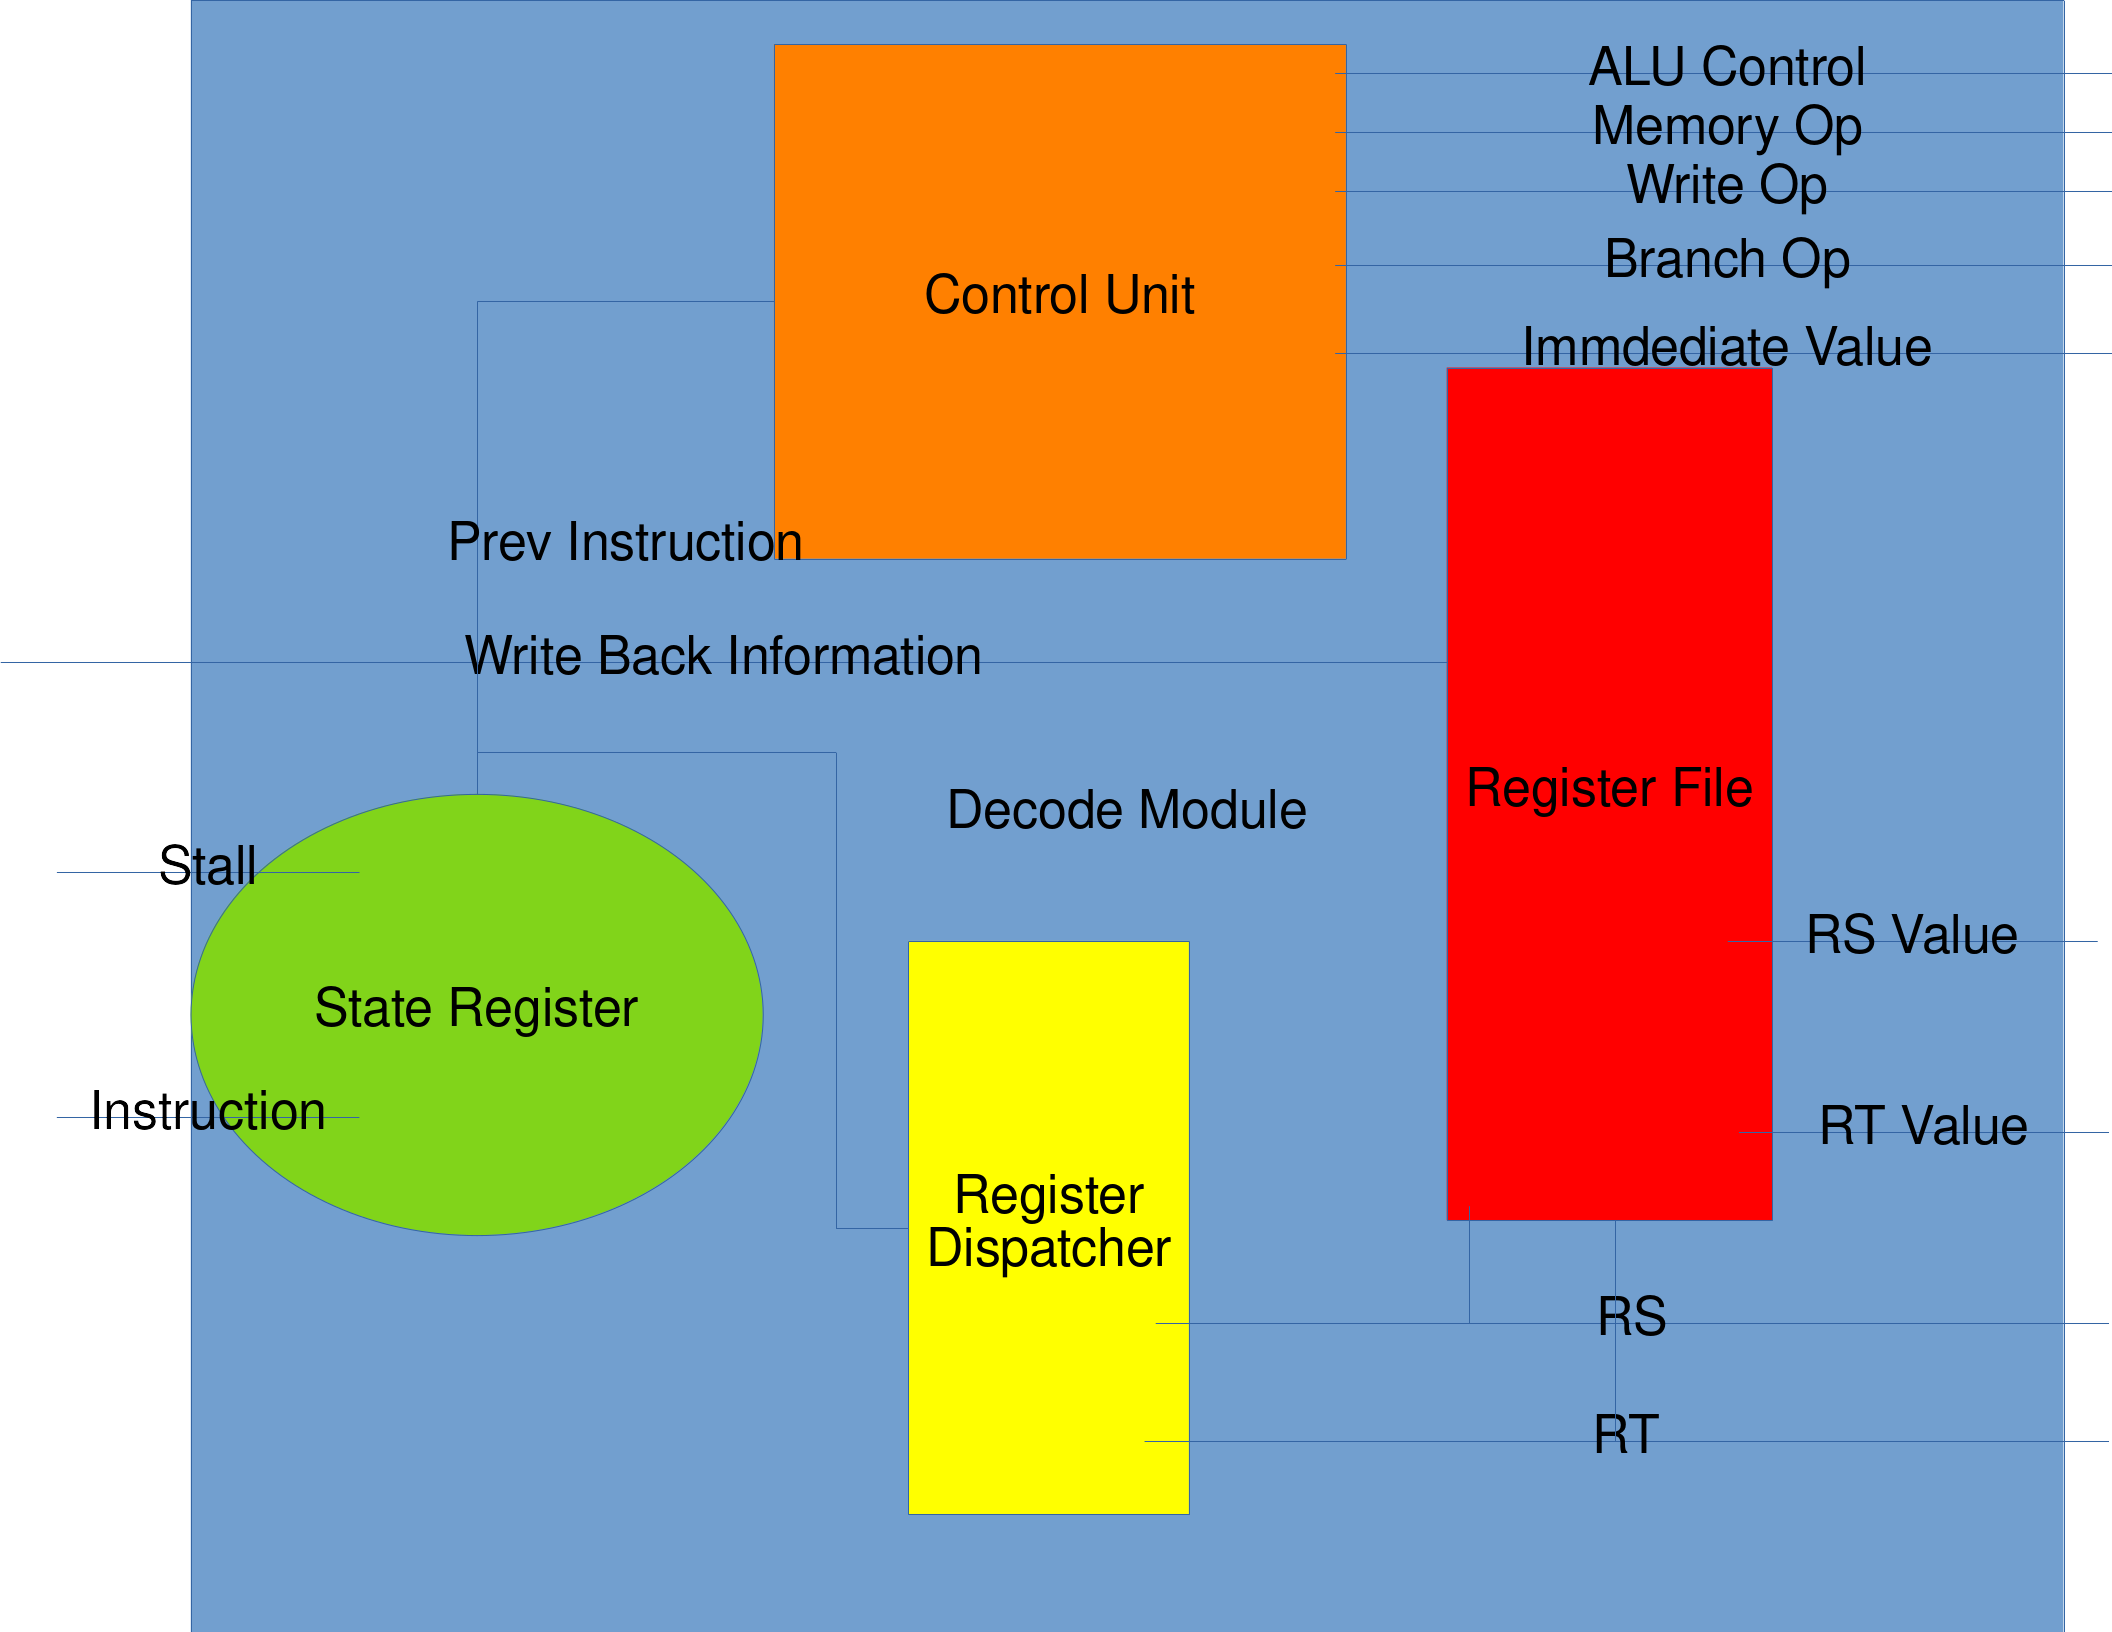
\includegraphics[width=\linewidth]{dm}
	\caption{Decode Module Diagram}
\end{figure}
\subsection{Arithmetic Module}
Arithmetic Module is in charge of calculations. It will also check the branching condition and determine the target. Memory Operation cannot live without this module either, as the memory address is decided in this part.
\subsubsection{Data Types}
In order to make life easier, let us first define some data types:
\begin{itemize}
\item \mintinline{haskell}{MemoryOperation'}: This will be one of the output of this module. Previously, we have already defined \mintinline{haskell}{MemoryOperation}. This new data type is almost the same, but the write operation carries its writing value now as the value is ready after arithmetic operations.
\begin{minted}{haskell}
data MemoryOperation'
  = MemNone'
  | MemLoad'
  | MemWrite' (BitVector 32)
deriving (Generic)
deriving (NFDataX)
deriving (Show)
\end{minted}
\item  \mintinline{haskell}{ALUState}: just the same as the output product of the Decode Module.
\item  \mintinline{haskell}{ALUOutput}: a product type of the output of this module
\begin{minted}{haskell}
type ALUOutput
  = ( Maybe (Unsigned 5)  -- write register
    , MemoryOperation'    -- memory
    , BitVector 32        -- ALU result
    , Maybe (Unsigned 32) -- branch target
    )
\end{minted}
\end{itemize}
\subsubsection{ALU}
ALU is a combinatorial circuit within the CPU that handles most of the arithmetic works. Here, our ALU follows the control command sent from the Control Unit and apply the target operations on its operands. Apart from the arithmetic result, ALU will also generate some flags like zero, negative and overflow. Although only zero flag is useful for this book, we are going to implement all these flags. 

For additions, overflow happens if the operands has the same sign bit while the sign bit differs in the result; for subtraction, overflow happens if the operands has different sign bit while the sign bit of the result is the same as the second operand. The following functions implement the detection of overflow:
\begin{minted}{haskell}
addOverflow :: BitVector 32 -> BitVector 32 -> (BitVector 32, Bool)
addOverflow a b =
  let c = a + b
  in (c, (a ! 31) == (b ! 31) && (a ! 31) /= (c ! 31))

subOverflow :: BitVector 32 -> BitVector 32 -> (BitVector 32, Bool)
subOverflow a b =
  let c = a - b
  in (c, (a ! 31) /= (b ! 31) && (c ! 31) == (b ! 31))
\end{minted}

The interface of ALU is described as the following:
\begin{minted}{haskell}
type ALUResult
  = ( BitVector 32 -- Arithmetic Result
    , Bool -- Overflow Result
    , Bool -- Zero Flag
    , Bool -- Negative Flag
    )

{-# ANN arithmeticUnit
    ( Synthesize
      { t_name = "ArithmeticUnit"
      , t_inputs =
          [ PortName "OPERATION"
          , PortName "OPERAND_1"
          , PortName "OPERAND_2"
          ]
      , t_output =
          PortProduct "ALU"
            [ PortName "RESULT"
            , PortName "OVERFLOW"
            , PortName "ZERO"
            , PortName "NEG"
            ]
       }
     )
#-}

arithmeticUnit :: ALUOperation -> BitVector 32 -> BitVector 32 -> ALUResult
arithmeticUnit op opr0 opr1 = (res, o, z, n)
  where
    (res, o, n) = arithmeticUnit' op
    z = res == 0
\end{minted}
The following part is the inner implementation of each operation:
\begin{enumerate}
	\item Addition and Subtraction: signed and unsigned addition change the bits in the same way, but only signed operation may overflow. 
	\begin{minted}{haskell}
arithmeticUnit' (ALUAdd flag) =
  let (res, overflow) = addOverflow opr0 opr1
  in (res, overflow && flag, bitToBool $ res ! 31)
arithmeticUnit' (ALUSub flag) =
  let (res, overflow) = subOverflow opr0 opr1
  in (res, overflow && flag, bitToBool $ res ! 31)
	\end{minted}
	\item And, Or, Xor, Nor are simple bitwise operations:
	\begin{minted}{haskell}
arithmeticUnit' ALUAnd = (opr0 .&. opr1, False, False)
arithmeticUnit' ALUNor = (complement $ opr0 .|. opr1, False, False)
arithmeticUnit' ALUOr  = (opr0 .|. opr1, False, False)
arithmeticUnit' ALUXor = (opr0 `xor` opr1, False, False) 
	\end{minted}
	\item Set-on-less-than needs to distinguish the sign information:
    \begin{minted}{haskell}
arithmeticUnit' (ALUSet flag) =
  let result =
    boolToBV $
      if flag
      then (unpack opr0 :: Signed 32)   < (unpack opr1 :: Signed 32)
      else (unpack opr0 :: Unsigned 32) < (unpack opr1 :: Unsigned 32)
  in (result, False, False)
\end{minted}
\item Shift operations can use the predefined functions in Clash but we need to check the sign information for the right shifting:
\begin{minted}{haskell}
arithmeticUnit' ALUShiftL =
  (opr0 `shiftL` (unpack $ extend opr1), False, False)
arithmeticUnit' (ALUShiftR True) =
  ( pack $ (unpack opr0 :: Signed 32) `shiftR` (unpack $ extend opr1)
  , False
  , False)
arithmeticUnit' (ALUShiftR False) =
  (opr0 `unsafeShiftR` (unpack $ extend opr1), False, False)
\end{minted}
\item Non-Operation does nothing:
\begin{minted}{haskell}
arithmeticUnit' ALUNone = (0, False, False)
\end{minted}
\end{enumerate}

\subsubsection{Forward Unit}
As we have mentioned, we must handle some data hazards using the forward strategy. This is done in the Forward Unit of Arithmetic Module.
\begin{minted}{haskell}
type ForwardInfo = Maybe (Unsigned 5, BitVector 32)

forwardUnit' 
  :: HiddenClockResetEnable dom
  => Signal dom ForwardInfo     -- mem register
  -> Signal dom ForwardInfo     -- write-back register
  -> Signal dom (Unsigned 5)    -- rs
  -> Signal dom (Unsigned 5)    -- rt
  -> Signal dom (Maybe (BitVector 32), Maybe (BitVector 32))
forwardUnit' a b c d = forwarding <$> a <*> b <*> c <*> d
  where
    forwarding exec load rs rt =
      let rs' =
             case (exec, load) of
               (Just (no, res), _)
                 | no == rs -> Just res
               (_, Just (no, res))
                 | no == rs -> Just res
               _            -> Nothing
          rt' =
             case (exec, load) of
               (Just (no, res), _)
                 | no == rt -> Just res
               (_, Just (no, res))
                 | no == rt -> Just res
               _            -> Nothing
       in (rs', rt')

{-# ANN forwardUnit
    ( Synthesize
      { t_name = "ForwardUnit"
      , t_inputs =
          [ PortName "CLOCK"
          , PortName "RESET"
          , PortName "ENABLE"
          , PortName "FORWARD_A"
          , PortName "FORWARD_B"
          , PortName "RS"
          , PortName "RT" 
          ]
      , t_output =
          PortProduct "FW" 
            [ PortName "OVERRIDE_RS"
            , PortName "OVERRIDE_RT"
            ]
      }
    )
#-}
forwardUnit 
  :: Clock System
  -> Reset System
  -> Enable System
  -> Signal System ForwardInfo    -- memm register
  -> Signal System ForwardInfo    -- load register
  -> Signal System (Unsigned 5)   -- rs
  -> Signal System (Unsigned 5)   -- rt
  -> Signal System (Maybe (BitVector 32), Maybe (BitVector 32))
forwardUnit = exposeClockResetEnable forwardUnit'
\end{minted}
This unit has two ports to accept forward data and two ports to get the register numbers. The forward data comes from two successor stages: memory stage and write-back stage; whenever there is a write-back request being issued in these two stages, it will be sent to the Forward Unit. If the write-back register happens to be the same as the operand register in ALU, then the data hazard is found. What if memory stage and write-back stage changes the same register? Notice that the changes in the write-back are already applied to the memory part by a previous forward, thus we can just accept the forward in the write-back part to get the latest value of the register. This handling method is expressed in the pattern matching order at the code above.

\subsubsection{State Machine}
The state transition of this module is also simple: when stalling happens, it just flushes away the current operations and states; otherwise, pulls out the operations from the current state and stores the new state.
\begin{minted}{haskell}
arithmeticModuleState' :: (ALUState, Bool) -> State ALUState ALUState
arithmeticModuleState' (_, True) = do
  let res
    = (Nothing, MemNone, NoBranch, ALUNone, Nothing, 0, 0, 0, 0, 0)
  put res
  return res
arithmeticModuleState' (state, False) = do
  res <- get
  put state
  return res

arithmeticModuleState 
  :: HiddenClockResetEnable dom
  => Signal dom (ALUState, Bool)
  -> Signal dom ALUState
arithmeticModuleState =
  asStateM arithmeticModuleState' 
    (Nothing, MemNone, NoBranch, ALUNone, Nothing, 0, 0, 0, 0, 0)
\end{minted}
\subsubsection{Arithmetic Module Interface}
Arithmetic Module has the most complicated logic relation. It must check a lot of things and do the arithmetic operations.
\begin{minted}[breaklines, linenos]{haskell}
{-# ANN arithmeticModule
    ( Synthesize
      { t_name = "AithmeticModule"
      , t_inputs =
          [ PortName "CLOCK"
          , PortName "RESET"
          , PortName "ENABLE"
          , PortName "FW_0"
          , PortName "FW_1"
          , PortName "STALL"
          , PortProduct "AM"
              [ PortName "WRITE"
              , PortName "MEM"
              , PortName "BRANCH_FLAG"
              , PortName "ALU"
              , PortName "IMM"
              , PortName "RS"
              , PortName "RSV"
              , PortName "RT"
              , PortName "RTV"
              , PortName "COUNTER"
              ]
          ]
      , t_output =
          PortProduct "AM"
            [ PortName "WRITE_REG"
            , PortName "MEM_OP"
            , PortName "RESULT"
            , PortName "BRANCH_TARGET"
            ]
      }
    )
#-}
arithmeticModule 
  :: Clock System
  -> Reset System
  -> Enable System
  -> Signal System ForwardInfo -- last
  -> Signal System ForwardInfo -- last last
  -> Signal System Bool
  -> Signal System ALUState    -- input
  -> Signal System ALUOutput   -- output
arithmeticModule clk rst enable last last' stall input =
  let (write, mem, branch, alu, imm, rs, rsv, rt, rtv, counter) =
        unbundle $
        ((exposeClockResetEnable arithmeticModuleState) clk rst enable) $
        bundle (input, stall)
      (check0, check1) = unbundle $ forwardUnit clk rst enable last last' rs rt
      
      unwrap (Just a) = a
      unwrap _ = 0
      
      rsv' = (<|>) <$> check0 <*> (pure <$> rsv)
      rtv0 = ((<|>) <$> check1 <*> (pure <$> rtv))
      rtv' = (<|>) <$> imm <*> rtv0
      
      memSolver MemWrite value = MemWrite' value
      memSolver MemLoad _ = MemLoad'
      memSolver _ _ = MemNone'
      
      mem' = memSolver <$> mem <*> (unwrap <$> rtv0)
      (res, _, z, _) =
        unbundle $
        arithmeticUnit <$> alu <*> (unwrap <$> rsv') <*> (unwrap <$> rtv')
      
      check_branch True (BranchEQ delta) pc _ = Just (pc + unpack delta)
      check_branch False (BranchNE delta) pc _ = Just (pc + unpack delta)
      check_branch _ Jump _ (Just i) = Just (unpack i)
      check_branch _ _ _ _ = Nothing
      
      branch' = check_branch <$> z <*> branch <*> counter <*> imm
  in bundle (write, mem', res, branch')
\end{minted}
Indeed, this module has a lot of things to do. 
\begin{enumerate}
	\item Line 44 to line 47 finish the state transition. 
	\item Line 48 checks the forwarding information.
	\item Line 53 to line 55 determines different register values. For RS, if there is a forward value, we will override the value to the latest version; For RT, we do mostly the same, but for the Arithmetic Unit, if there is an immediate value, the final value should be \mintinline{haskell}{rtv'}; but RT can also be used in the output of memory operation flags for the next stage, in that case, we will use \mintinline{haskell}{rt0}.
	\item Line 57-61 decides the memory flags and values.
	\item Line 62-64 represents the ALU operations.
	\item Line 66-71 checks branching/jumping and calculates the target.
\end{enumerate}
\begin{figure}[H]
	\centering
	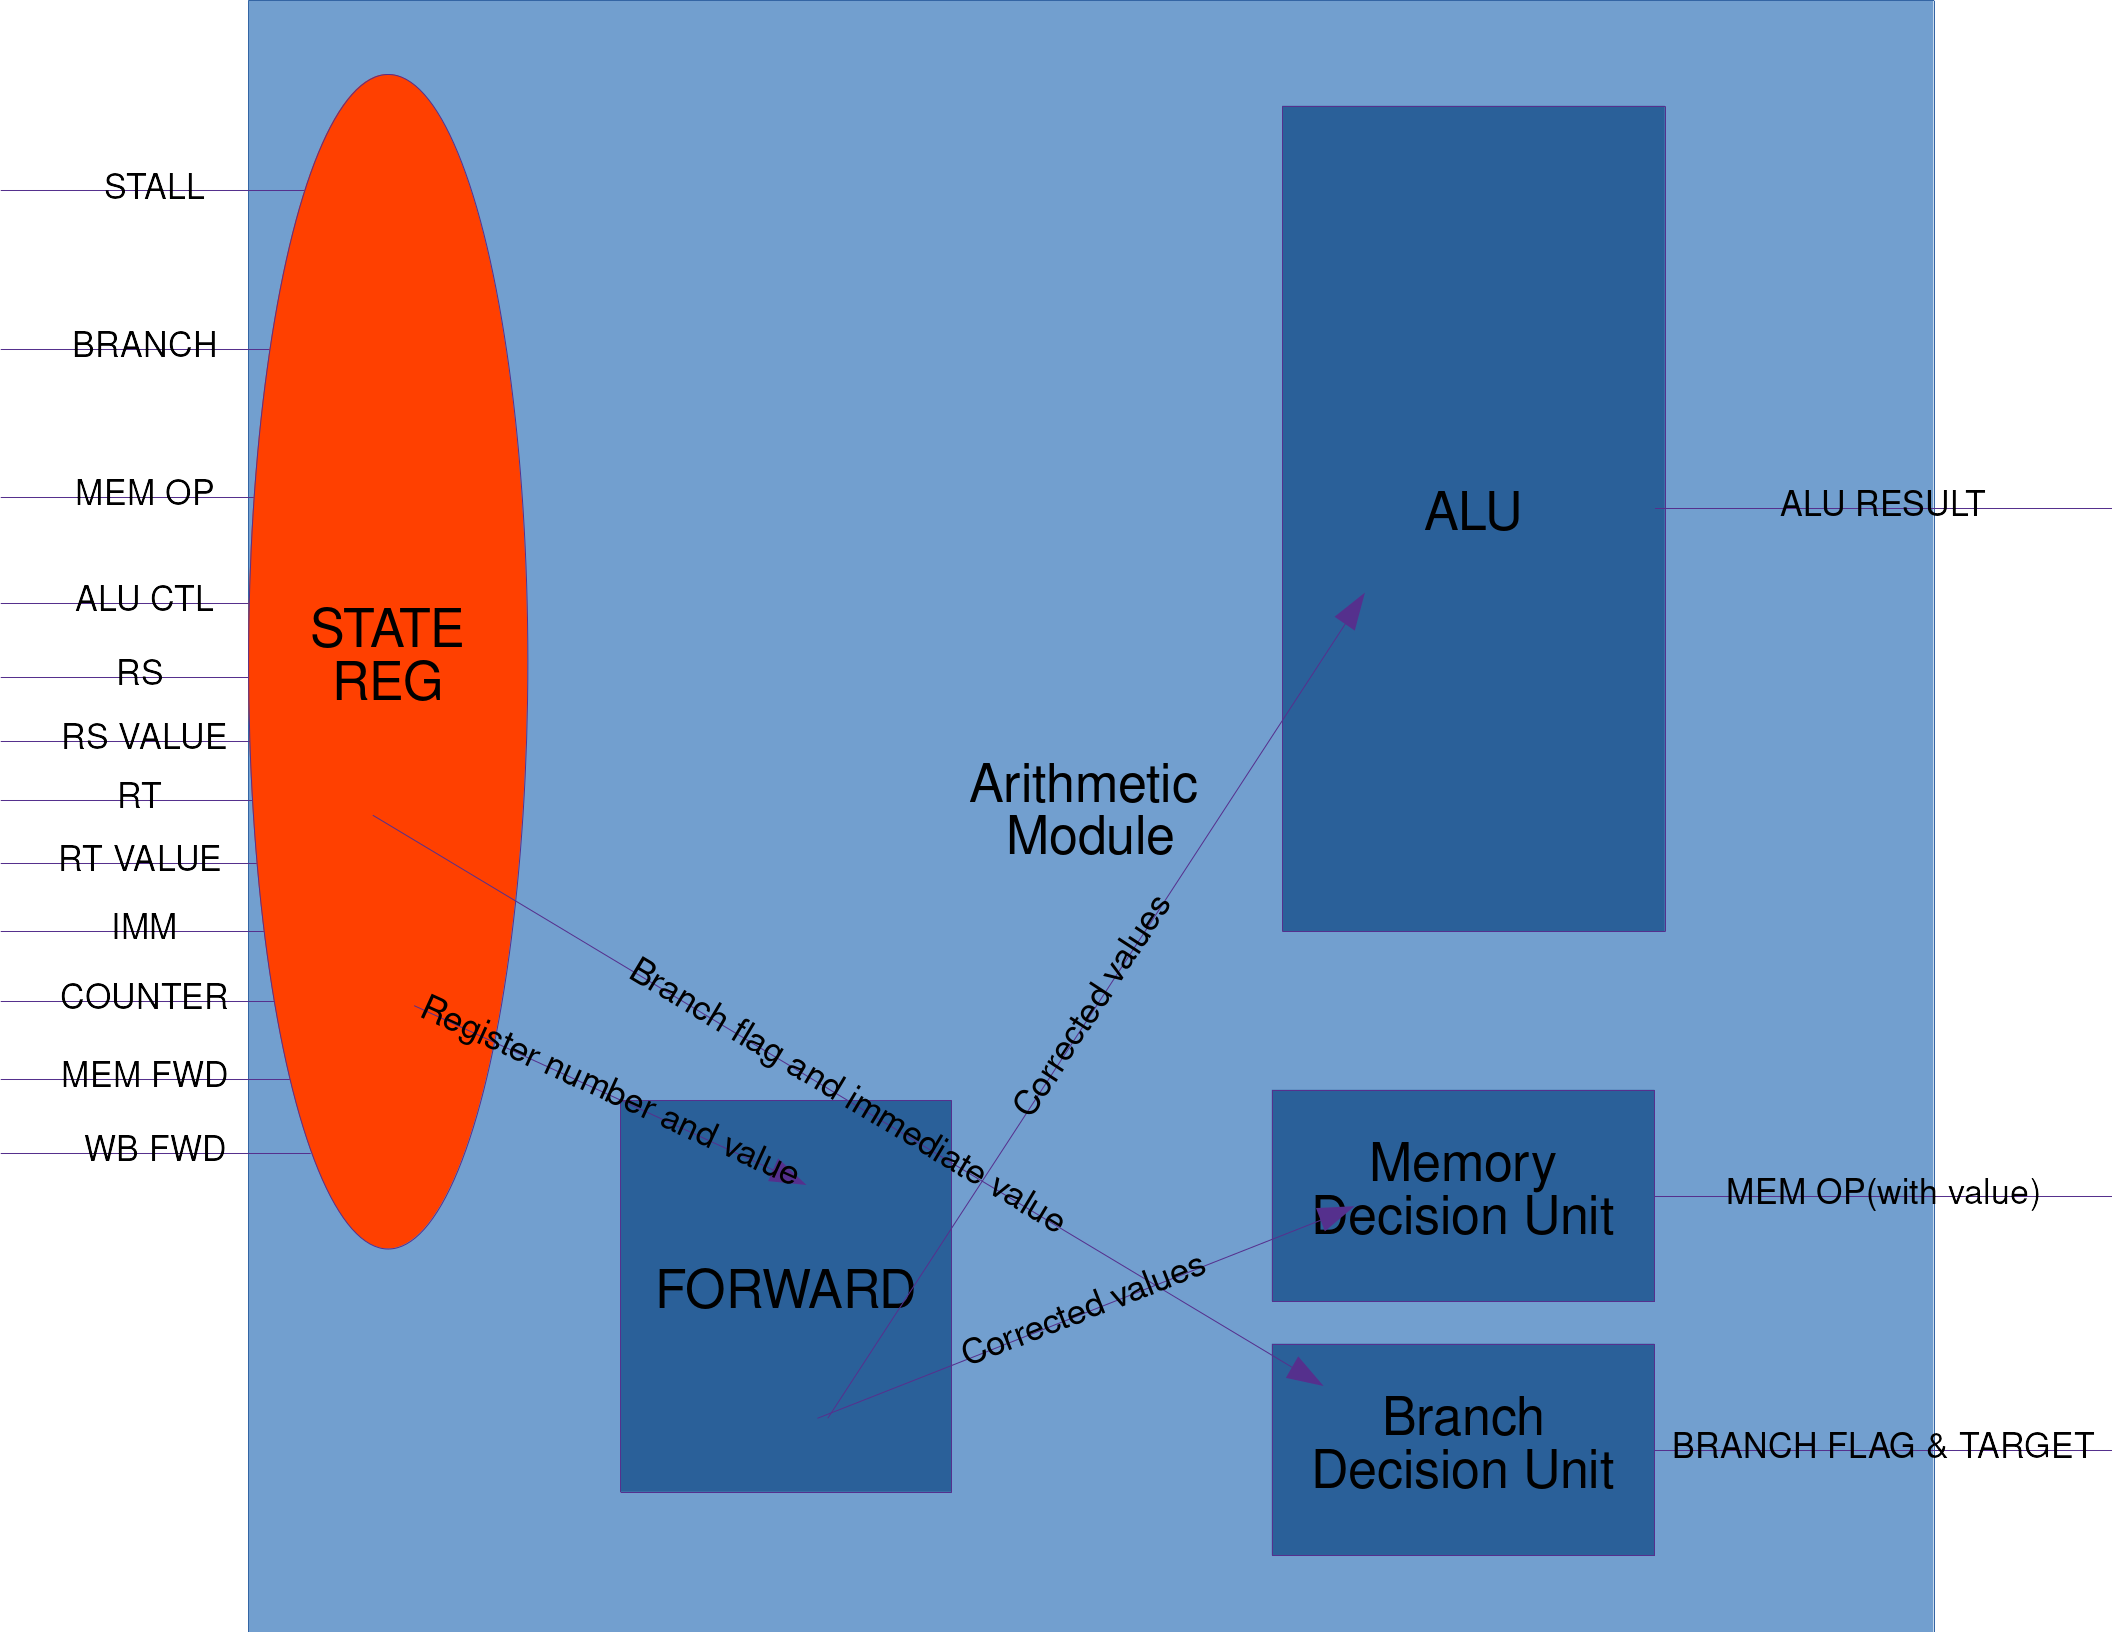
\includegraphics[width=\linewidth]{am}
	\caption{Arithmetic Module Diagram)}
\end{figure}
\subsection{Memory Module}
\subsubsection{Main Memory Block}
The main memory also uses the BRAM structure. It is implemented in the following:
\begin{minted}[breaklines, linenos]{haskell}
{-# ANN mainRAM
    ( Synthesize
      { t_name = "MainMemory"
      , t_inputs =
          [ PortName "CLOCK"
          , PortName "RESET"
          , PortName "ENABLE"
          , PortName "FETCH_ADDRESS"
          , PortName "EDIT_SERIAL"
          ]
      , t_output = PortName "DATA"
      }
    )
#-}

mainRAM 
  :: Clock  System
  -> Reset  System
  -> Enable System
  -> Signal System MemAddr
  -> Signal System (Maybe (MemAddr, MemoryBlock))
  -> Signal System MemoryBlock
mainRAM = exposeClockResetEnable $ blockRam (replicate d512 0)
\end{minted}
The block memory adapts the default write-after-read strategy and it takes two inputs: the read address and the write information. 
\subsubsection{Memory State}
Again, the state transition is mainly about exchange the output data from the previous module.
\begin{minted}[breaklines, linenos]{haskell}
memState' :: (ALUOutput, Bool) -> State ALUOutput ALUOutput
memState' (_, True) = do
  let res = (Nothing, MemNone', 0, Nothing)
  put res
  return res
memState' (state, _) = do
  res <- get
  put state
  return res

memState 
  :: HiddenClockResetEnable dom
  => Signal dom (ALUOutput, Bool)
  -> Signal dom ALUOutput
memState = asStateM memState' (Nothing, MemNone', 0, Nothing)
\end{minted}
\subsubsection{Memory Module Interface}
\begin{minted}[breaklines, linenos]{haskell}
type MemOutput
  = ( Maybe (Unsigned 32) -- branch target
    , Maybe (RegNo, Reg)  -- write pair
    )

{-# ANN memoryModule
    ( Synthesize
      { t_name = "MemoryModule"
      , t_inputs =
          [ PortName "CLOCK"
          , PortName "RESET"
          , PortName "ENABLE"
          , PortProduct "MMI"
              [ PortName "WRITE_REG"
              , PortName "MEM_OP"
              , PortName "RESULT"
              , PortName "BRANCH_TARGET"
              ]
          , PortName "STALL"
          ]
      , t_output =
          PortProduct "MMO" 
            [ PortName "BRANCH"
            , PortName "WRITE_PAIR"
            ]
      }
   )
#-}
memoryModule 
  :: Clock System
  -> Reset System
  -> Enable System
  -> Signal System ALUOutput
  -> Signal System Bool
  -> Signal System MemOutput
memoryModule clk rst enable aluOut stall =
  let stateMachine = 
        (exposeClockResetEnable memState) clk rst enable
      (writeReg,  memOpPrev, aluRes, br) =
        unbundle $ stateMachine $ bundle (aluOut, stall)

      writeInfoSolver _ _ True _ = Nothing
      writeInfoSolver address (MemWrite' v) _ Nothing = 
        Just (unpack address, v)
      writeInfoSolver _ _ _ _ = Nothing

      thirdData  (_, _, x, _) = x `unsafeShiftR` 2
      secondData (_, x, _, _) = x

      aluRes' = thirdData <$> aluOut
      memOp   = secondData <$> aluOut

      writeInfo = 
        writeInfoSolver 
          <$> aluRes'<*> memOp <*> stall <*> br

      memData = 
        mainRAM clk rst enable (unpack <$> aluRes') writeInfo

      writePair (Just no) _ MemLoad' res = Just (no, res)
      writePair (Just no) res _ _ = Just (no, res)
      writePair _ _ _ _ = Nothing

      writePair' = 
        writePair 
          <$> writeReg <*> aluRes <*> memOpPrev <*> memData

      check True _ = (Nothing, Nothing)
      check _ x = x
  in check <$> stall <*> bundle (br, writePair')
\end{minted}
Please notice that \mintinline{haskell}{aluRes'} and \mintinline{haskell}{memOp} comes from the Arithmetic Module at the same cycle, this makes sure that in the next cycle, the BRAM will output the correct data.

The memory read/write information is derived from the instant input while the register write information comes from the state register; this prevents possible oscillations and fits well with the BRAM delay effects.
\begin{figure}[H]
	\centering
	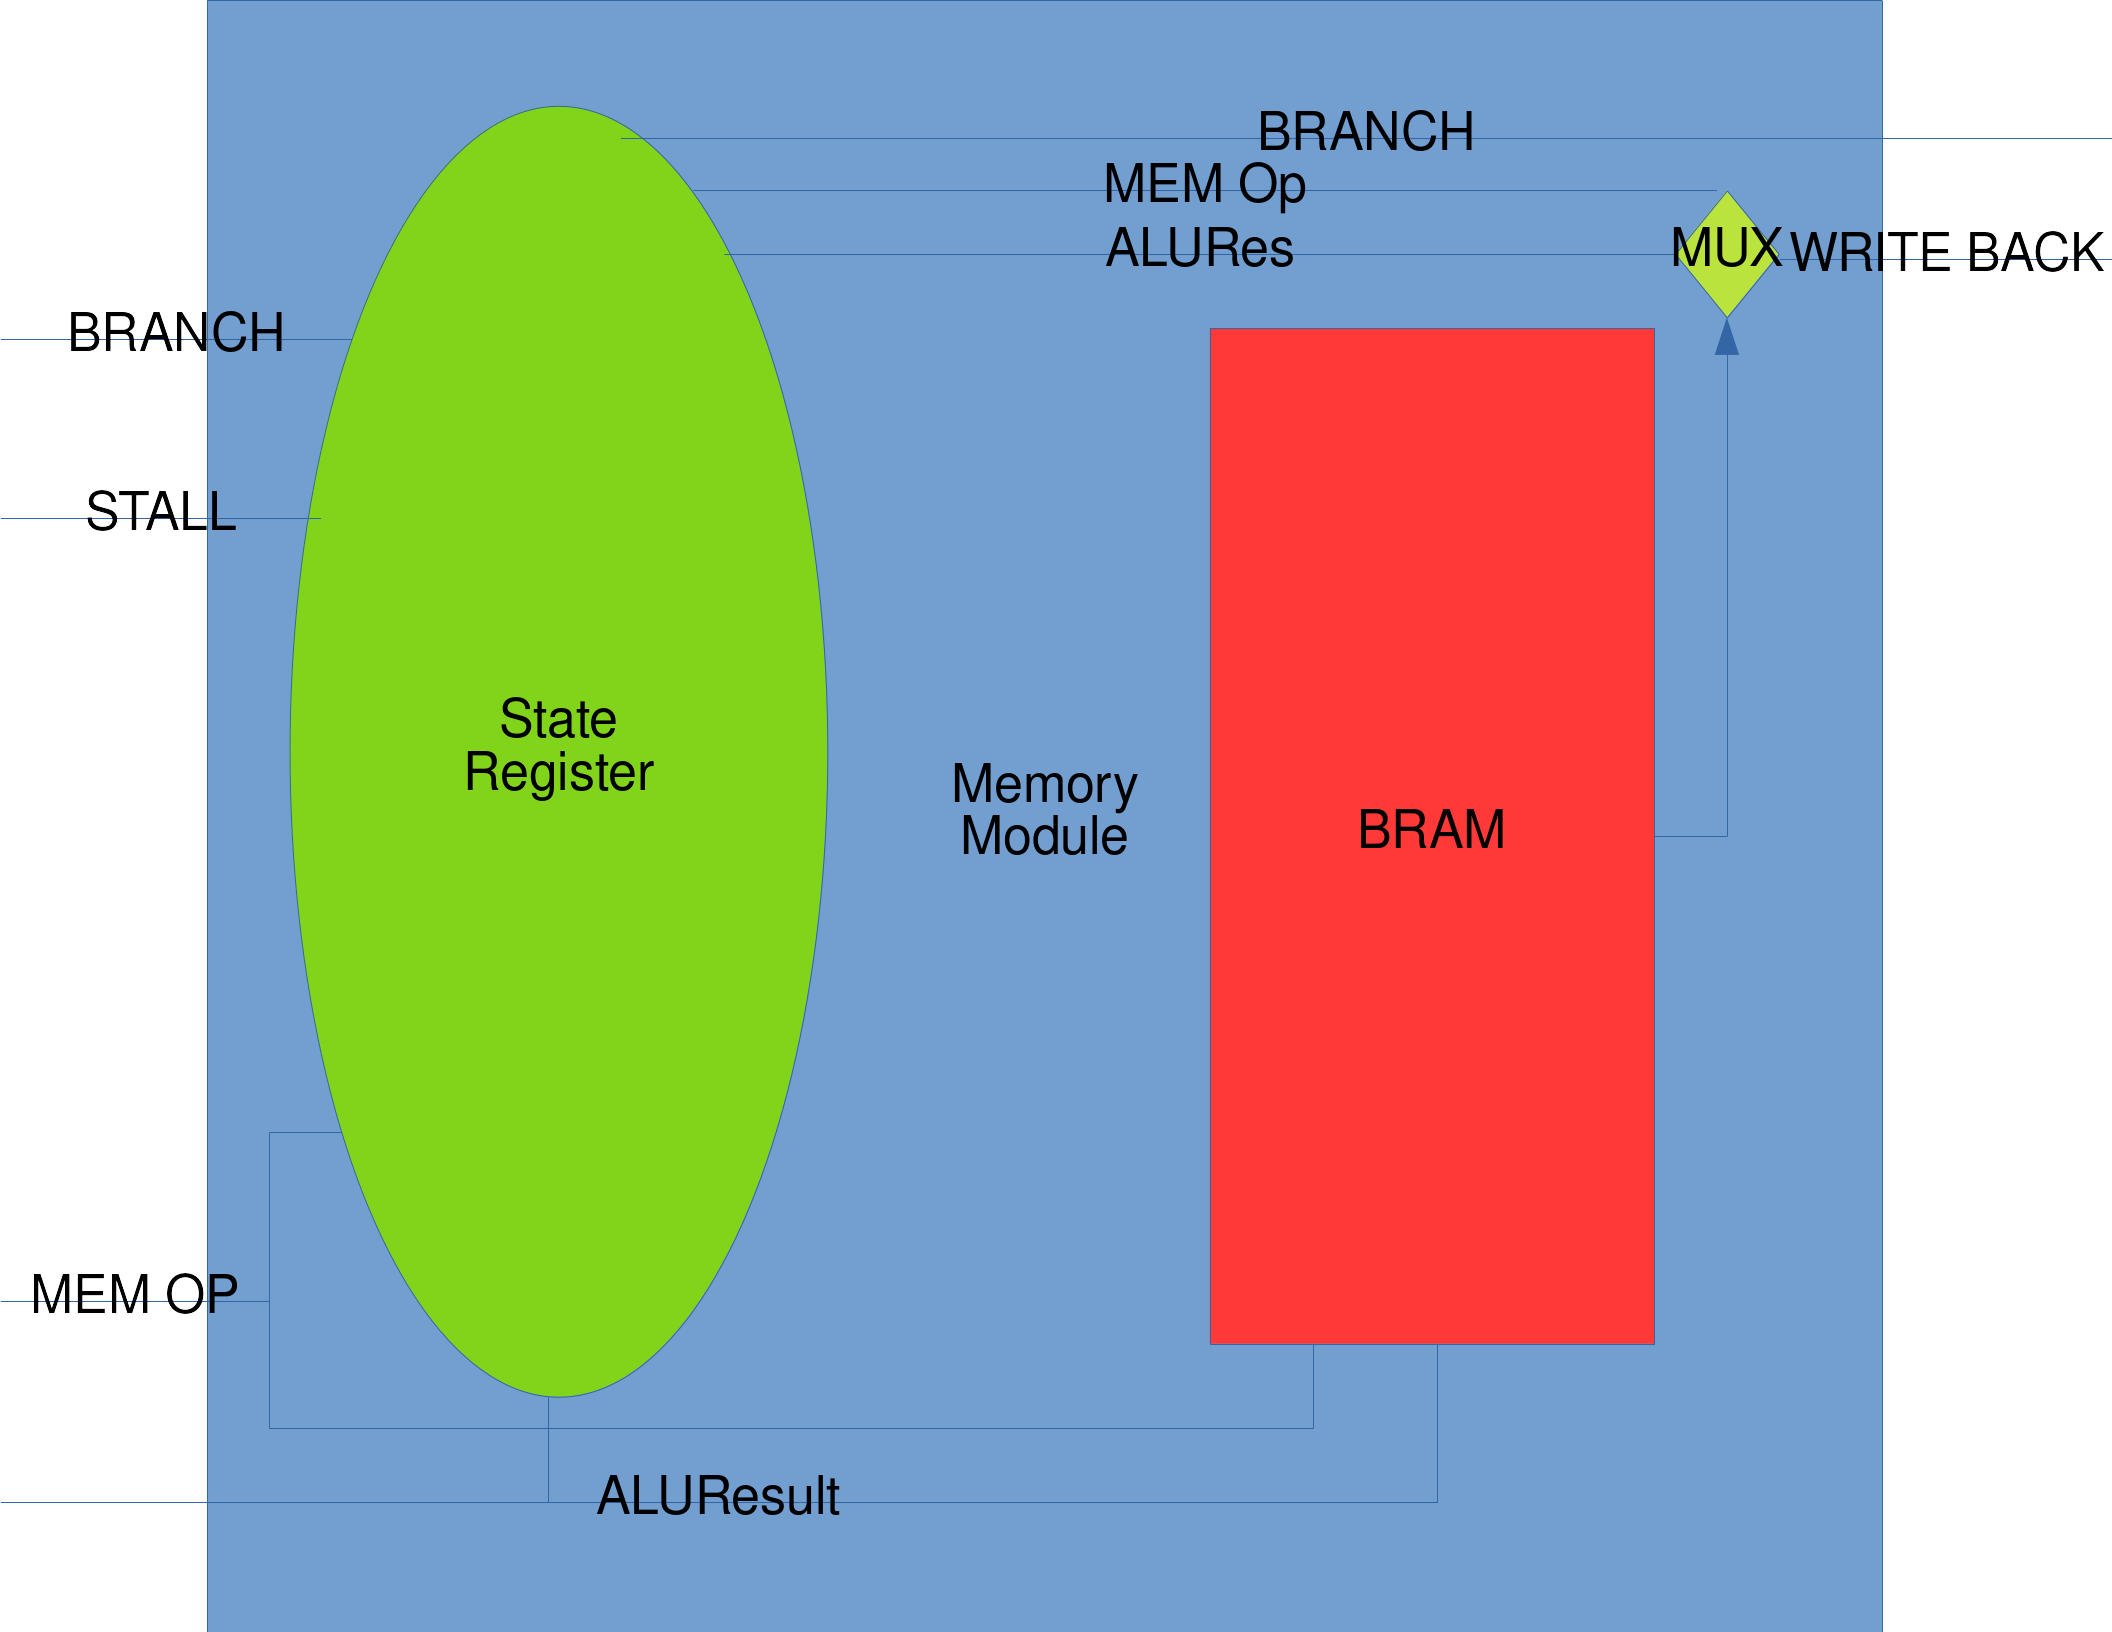
\includegraphics[width=\linewidth]{mm}
	\caption{Memory Module Diagram}
\end{figure}
\subsection{Write-Back Module}
Write-Back is the simplest module: just a buffer before editing the data.
\subsubsection{State Register}
The state of this module is simply a register. In this part, we do not need to care about stalling.
\begin{minted}[breaklines, linenos]{haskell}
writeRegister 
  :: HiddenClockResetEnable dom
  => Signal dom (Maybe (Unsigned 32), Maybe (RegNo, Reg))
  -> Signal dom (Maybe (Unsigned 32), Maybe (RegNo, Reg))
writeRegister = register (Nothing, Nothing)
\end{minted}
\subsubsection{Write-Back Module Interface}
The interface is nothing more than a wrapper around the register:
\begin{minted}[breaklines, linenos]{haskell}
{-# ANN writeBack
  ( Synthesize 
    { t_name = "WriteBack"
    , t_inputs =
        [ PortName "CLOCK"
        , PortName "RESET"
        , PortName "ENABLE"
        , PortName "BRANCH"
        , PortName "WRITE_PAIR"
        ]
    , t_output =
        PortProduct "WB" 
          [ PortName "BRANCH"
          , PortName "WRITE_PAIR"
          ]
    }
  )
#-}
writeBack 
  :: Clock System
  -> Reset System
  -> Enable System
  -> Signal System (Maybe (Unsigned 32))
  -> Signal System (Maybe (RegNo, Reg))
  -> Signal System (Maybe (Unsigned 32), Maybe (RegNo, Reg))
writeBack clk rs en br wb = writeRegister' $ bundle (br, wb)
  where
    writeRegister' = (exposeClockResetEnable writeRegister) clk rs en
\end{minted}